% "Brief" explanation of the Schwarz-Christoffel transform
% David Lawrence Miller
% d.l.miller@bath.ac.uk

% Started : 29 October 2008

\documentclass[a4paper,10pt]{amsart}

% Load some packages
\usepackage{times, amsmath, amssymb, amsfonts, url, natbib, bm, rotating}

\usepackage{multirow}
\usepackage{graphicx}

% top matter
\title{a title}
\author{David Lawrence Miller}
\email{d.l.miller@bath.ac.uk}
\address{Mathematical Sciences, University of Bath, Bath, United Kingdom}

% Shortcuts
% Probability
\newcommand{\prob}[1]{\mathbb{P}\left[ #1 \right]}
% Hovitz-Thompson
\newcommand{\HT}{\hat{\tau}_{HT}}
% Schwarz-Christoffel
\newcommand{\sch}{Schwarz-Christoffel }
% fprime
\newcommand{\fprime}{f^\prime(z)}

\begin{document}

% The abstract
\begin{abstract}
abstract from useR?
\end{abstract}


% New theorem for theorems
\newtheorem{thm}{Theorem}[section]

%New theorem for definitions
\newtheorem{defn}{Definition}[section]

\maketitle



\section{Ramsey's horseshoe}

\ref{ramsay} proposes a function which can be used to benchmark new approaches to 2-dimensional smoothing. The function takes the form of a horseshoe which is flat across the domain but ranges from $-4$ to $4$ along the domains long axis. The so-called ``Ramsay horseshoe'' is shown in \ref{ramsayshorseshoe}.

Problems occur when the smooth uses the Euclidean distance between the $4$ and $-4$ arms of the hoseshoe. Clearly within the area the distance between these points is large, however instead we smooth across these features and observe a phenomenon known as ``leakage''. This clearly gives rise to bias in the inside of the horseshoe.


\begin{table}
\centering
\begin{tabular}{c}
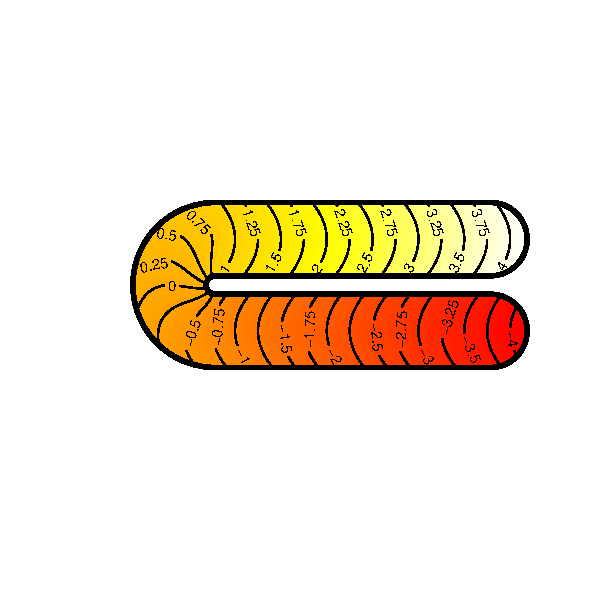
\includegraphics[scale=0.25]{figs/ramsayhorseshoe.pdf} \\
\end{tabular}
\caption{Heatmap of the Ramsay horseshoe.}
\label{rtest}
\end{table}

Clearly we would like to use an approach that respects the shape of the region and does not show any evidence of leakage. In order to deal with the problems of a complex region, four different approaches have been proposed:

\begin{enumerate}
\item \cite{ramsay} proposes finite area $L$-splines (FELSPLINEs) which consist of triangulating the domain and then constructs a bivariate quadratic polynomial basis functions over each triangle, specifying that there be continuity over the edges of the triangles. The union of these functions is then a solution to a PDE.

The problem with FELSPLINE is that it must have that the gradient is normal to the edge of the area. This is not neccessarily physically realistic in all situations.

\item \cite{wangranalli} adopt a ``within-area distance'' formulation for thin plate splines. In this case they take the geodesic distance between two points, that being the shortest path within the domain in order to address the problem of the definition of ``close'' in the domain. 

\item \cite{soap} consider a soap film over the domain which is weighed down by the data whilst minimizing the surface tension in the film.

\item An alternative approach is to ``morph'' the area in question to be one that is more suitable for smoothing upon. This is what we propose here.

\end{enumerate}




\section{Method}

Here we formulate a conformal mapping from the domain of the problem (we call this the $W$ domain) to a domain on which it is easier to smooth (and where we can avoid the problems detailed above.)

\subsection{\sch}


\subsection{Problems}

Linear fit onto the horseshoe.
Look at some other shapes that break it.



\subsection{Procedure}

Our procedure consists of the following steps:

\begin{enumerate}
\item Determine the area over which we would like to smooth, $W$.

\item Compute the \sch transform of $W$ to get $Z$.

\item Map the co-ordinates of the datapoints in $W$ to $Z$.

\item Fit the GAM to the data in $Z$.

\end{enumerate}

Say something about:
Doing analysis in $Z$, doing analysis in $W$.




Brief bit about SC.

Algorithm that we use.

Matlab+R approach.



\section{Simulations}

What do we want to look at?

Why p-splines?


\section{Analysis}


Linear model stuff, will this work elsewhere?














\bibliographystyle{plainnat}
\bibliography{sc-refs}



\end{document}
